% Paper 99 — CRMLint: Automated Logical Cost Analysis of Mathematical Proof
% Paper 99, of the Constructive Reverse Mathematics Series
% Paul Chun-Kit Lee, 2026
%
% This is a methodological paper in six parts.  It does not follow the
% standard CRM series template.

\documentclass[11pt,a4paper]{article}

% ── packages ──────────────────────────────────────────────────────────
\usepackage[utf8]{inputenc}
\usepackage[T1]{fontenc}
\usepackage{amsmath,amssymb,amsthm,mathtools}
\usepackage{hyperref}
\usepackage{enumitem}
\usepackage{booktabs}
\usepackage{array}
\usepackage{longtable}
\usepackage{xcolor}
\usepackage{tikz}
\usetikzlibrary{positioning,arrows.meta,calc,patterns,decorations.pathreplacing}
\usepackage[margin=1in]{geometry}
\usepackage{fancyhdr}
\usepackage{titlesec}

% ── theorem environments ──────────────────────────────────────────────
\theoremstyle{plain}
\newtheorem{theorem}{Theorem}[section]
\newtheorem{lemma}[theorem]{Lemma}
\newtheorem{proposition}[theorem]{Proposition}
\newtheorem{corollary}[theorem]{Corollary}
\theoremstyle{definition}
\newtheorem{definition}[theorem]{Definition}
\newtheorem{example}[theorem]{Example}
\newtheorem{remark}[theorem]{Remark}
\newtheorem{observation}[theorem]{Observation}

% ── macros ────────────────────────────────────────────────────────────
\newcommand{\BISH}{\textup{BISH}}
\newcommand{\MP}{\textup{MP}}
\newcommand{\LLPO}{\textup{LLPO}}
\newcommand{\WKL}{\textup{WKL}}
\newcommand{\WLPO}{\textup{WLPO}}
\newcommand{\LPO}{\textup{LPO}}
\newcommand{\CLASS}{\textup{CLASS}}
\newcommand{\CRMlint}{\textsc{CRMlint}}
\newcommand{\R}{\mathbb{R}}
\newcommand{\Z}{\mathbb{Z}}
\newcommand{\N}{\mathbb{N}}
\newcommand{\Q}{\mathbb{Q}}
\newcommand{\C}{\mathbb{C}}
\newcommand{\Lean}{\textsc{Lean\,4}}
\newcommand{\Mathlib}{\textsc{Mathlib4}}
\newcommand{\LTE}{\textup{LTE}}

% ── formatting ────────────────────────────────────────────────────────
\titleformat{\part}[display]
  {\centering\Large\bfseries}{Part \thepart}{12pt}{\LARGE}
\titleformat{\section}{\large\bfseries}{\thesection}{1em}{}
\pagestyle{fancy}
\fancyhf{}
\fancyhead[L]{\small Paper 99 — CRMLint}
\fancyhead[R]{\small CRM Series}
\fancyfoot[C]{\thepage}

% ══════════════════════════════════════════════════════════════════════
\begin{document}

\title{\textbf{CRMLint: Automated Logical Cost Analysis of Mathematical Proof}\\[6pt]
\large Paper 99, of the Constructive Reverse Mathematics Series\\[3pt]
\normalsize A Methodological Paper in Six Parts}

\author{Paul Chun-Kit Lee\\
\small Division of Cardiology, NYU Grossman School of Medicine\\
\small \texttt{paul.lee@nyulangone.org}}

\date{March 2026}

\maketitle

\begin{abstract}
We describe the design, calibration, and first external deployment of
\CRMlint, a heuristic tool for estimating the constructive reverse
mathematics (CRM) signature of mathematical proofs.  \CRMlint\ operates
in three modes: as a Lean~4 proof-term analyzer, as a structural proof
profiler, and as a lightweight LaTeX scanner that classifies papers by
keyword and citation pattern matching.

Calibration against 627 declarations across 10 \Mathlib\ files recovers
the expected algebraic/analytic divide: 92.0\% of declarations are
$\BISH$, with classical content concentrating in inner product spaces
and convergence arguments.  A three-axis structural analysis finds
that Archimedean proofs are $1.4\times$ more complex, $2.8\times$ deeper
in dependency chains, and carry $4.3\times$ more external lemma
invocations than their non-Archimedean counterparts.

We deploy the LaTeX scanner against the 15-file blueprint of the
Liquid Tensor Experiment (LTE), Scholze's formally verified proof of
Theorem~9.4 on Ext-vanishing for $p'$-liquid real vector spaces.  The
initial scan returns 86.7\% $\BISH$---a gross undercount caused by
the scanner's inability to detect norm-comparison content that is
structurally present but does not match any keyword pattern.  We call
this \emph{Archimedean dark matter}.  Patching the dictionary to detect
norm-filtration patterns revises the profile to 33.3\% $\BISH$ /
66.7\% $\LPO$.

We then annotate the LTE's mathematical content---the main theorem,
its six-link proof chain, and the normed homological algebra toolkit---with
CRM levels at each step.  This is exposition, not discovery: the
concentration of classical content at norm-filtration gates is a design
feature of condensed mathematics, understood by its creators.  Our
contribution is a vocabulary (the CRM hierarchy provides a graduated
scale where before there was a binary algebra/analysis distinction) and
a tool (the scanner automates detection of this structure for proofs
where the architecture is not designed).

The paper is honest about what it does not contribute: no new
mathematics, no simplification of the LTE, no result that would
surprise Scholze.
\end{abstract}

\tableofcontents
\newpage


% ══════════════════════════════════════════════════════════════════════
%                           PART I
% ══════════════════════════════════════════════════════════════════════
\part{Genesis}\label{part:genesis}

\section{The problem}\label{sec:problem}

After 96 papers of manual CRM audit---classifying theorems one at a time,
tracing axiom dependencies by hand, flagging each use of excluded middle
or Archimedean completeness---the bottleneck in the program shifted from
mathematics to labor.  The CRM classification of a single theorem
(say, the Gross--Zagier formula) requires reading the proof, identifying
every appeal to a non-constructive principle, and tracing each appeal
to its minimal logical strength.  Papers~78--96 each took 2--5 days of
combined human and AI effort.  Scaling this to the full Mathlib library
(${\sim}200{,}000$ declarations as of early 2026) is infeasible by hand.

The question that opens this paper is operational: \emph{can the CRM
classification of a proof be automated?}

\section{What CRM measures}\label{sec:what-crm-measures}

CRM assigns to each proof a \emph{logical signature} $\sigma(P)$, the
weakest axiom system in which the proof can be carried out.  The
hierarchy is:
\[
  \BISH \;\subset\; \BISH{+}\MP \;\subset\; \BISH{+}\LLPO
  \;\subset\; \BISH{+}\WKL \;\subset\; \BISH{+}\WLPO
  \;\subset\; \BISH{+}\LPO \;\subset\; \CLASS
\]
A theorem with signature $\BISH$ requires no omniscience principle
whatsoever: every step is computationally witnessed.  A theorem with
signature $\CLASS$ invokes the full law of excluded middle somewhere
in its proof tree.  The intermediate levels---$\MP$, $\LLPO$, $\WKL$,
$\WLPO$, $\LPO$---measure calibrated degrees of non-constructivity,
each corresponding to a specific decision problem on infinite sequences
or real numbers.

The CRM signature is \emph{not} a measure of proof complexity.
Taylor--Wiles patching is technically intricate but logically $\WKL$
(an inverse limit of finite objects).  The intermediate value theorem
is elementary but logically $\WLPO$ (it requires deciding whether a
real number equals zero).  CRM measures the \emph{logical cost} of a
proof---the price paid for treating the continuum as a completed object
with decidable properties.

\section{Three generations of automation}\label{sec:three-gen}

\CRMlint\ was developed in three stages, each addressing a different
aspect of the automation problem:

\medskip
\noindent\textbf{Generation 1: Theoretical framework}
(\texttt{crmlint.py}, 1{,}161 lines).
Models the CRM hierarchy, six realization functors (Betti, de~Rham,
\'etale, crystalline, Hodge, automorphic) with their CRM costs,
comparison isomorphisms, and the Archimedean Obstruction Theorem of
Paper~98.  Proof DAGs compute signatures by max-propagation over
dependency edges.  A substitution database stores eight seed entries
extracted from Papers~50--97: known techniques where a classical method
can be replaced by a constructive alternative at lower logical cost.

This generation answers: \emph{what is the right mathematical model
for CRM signatures of composite proofs?}

\medskip
\noindent\textbf{Generation 2: Empirical validation}
(\texttt{crmlint\_crawler.py}, 653 lines;
\texttt{crmlint\_structure.py}, 793 lines).
The crawler fetches Lean~4 source files from \Mathlib\ on GitHub,
parses declarations, and heuristic-classifies each by CRM level using
tactic and keyword signatures (${\sim}40$ classical indicators including
\texttt{by\_contra}, \texttt{Classical.choice}, inner product space
infrastructure, integration, and topological convergence patterns).
The structure analyzer computes seven-dimensional proof profiles:
proof size (lines, tactic count), dependency depth (\texttt{have}/\texttt{let}
chains), proof width (active hypotheses, case splits), and modularity
(automation ratio, external lemma invocations, rewrite density).

This generation answers: \emph{does the CRM hierarchy correlate with
structural proof complexity in real Lean code?}

\medskip
\noindent\textbf{Generation 3: LaTeX scanner}
(\texttt{crmlint\_scanner.py}, 810 lines at v1.0, 870 lines at v1.1).
Keyword and citation pattern matching against ${\sim}90$ technique
markers and ${\sim}120$ landmark paper citations, applied directly to
\texttt{.tex} source.  No Lean, no LLM, no external dependencies
beyond the Python standard library.  Scans a directory of papers in
seconds.  Anti-marker patterns suppress false positives (e.g.,
algebraic ``integral closure'' is not analytic integration).

This generation answers: \emph{can we triage thousands of papers by
CRM cost before investing months in any one?}

\medskip

The three generations are complementary.  Generation~1 provides the
theory; Generation~2 tests it against ground truth; Generation~3
scales it to the full mathematical literature.  All three are
implemented in pure Python with zero external dependencies (3{,}417
lines total at v1.0).


% ══════════════════════════════════════════════════════════════════════
%                           PART II
% ══════════════════════════════════════════════════════════════════════
\part{Calibration: Mathlib at 627 Declarations}\label{part:mathlib}

\section{Target selection}\label{sec:target-selection}

We selected 10 \Mathlib\ files spanning eight mathematical domains:

\begin{center}
\small
\begin{tabular}{lll}
\toprule
\textbf{File} & \textbf{Domain} & \textbf{Decls} \\
\midrule
\texttt{EllipticCurve/Weierstrass.lean} & Algebraic Geometry & 68 \\
\texttt{InnerProductSpace/Basic.lean} & Analysis & 141 \\
\texttt{SpecificLimits/Basic.lean} & Analysis & 83 \\
\texttt{Galois/Basic.lean} & Field Theory & 61 \\
\texttt{Charpoly/Basic.lean} & Linear Algebra & 39 \\
\texttt{ArithmeticFunction.lean} & Number Theory & 0 \\
\texttt{Bernoulli.lean} & Number Theory & 27 \\
\texttt{RepresentationTheory/Basic.lean} & Representation Theory & 67 \\
\texttt{Cyclotomic/Basic.lean} & Ring Theory & 57 \\
\texttt{InfiniteSum/Basic.lean} & Topology & 84 \\
\bottomrule
\end{tabular}
\end{center}

The selection was guided by two criteria: (1)~coverage of the
algebraic/analytic divide that the Archimedean Obstruction Thesis
predicts to be the primary CRM boundary, and (2)~inclusion of domains
where the CRM series has ground-truth classifications from manual
audit (inner product spaces from Paper~77, elliptic curves from
Paper~95, Galois theory from Paper~78).

\section{Generation 2 results: the crawler}\label{sec:crawler-results}

The crawler classified 627 declarations:

\begin{center}
\begin{tabular}{lrrl}
\toprule
\textbf{CRM Level} & \textbf{Count} & \textbf{\%} & \\
\midrule
$\BISH$  & 577 & 92.0 & \rule{4.6cm}{6pt} \\
$\WKL$   &  11 &  1.8 & \rule{0.09cm}{6pt} \\
$\WLPO$  &  20 &  3.2 & \rule{0.16cm}{6pt} \\
$\CLASS$ &  19 &  3.0 & \rule{0.15cm}{6pt} \\
\bottomrule
\end{tabular}
\end{center}

The 92\% $\BISH$ figure is consistent with the programme's central
finding: most of mathematics, as actually practiced in a modern proof
library, is constructive.  The 8\% non-$\BISH$ content concentrates
in three locations:

\begin{enumerate}[label=(\roman*)]
\item \textbf{Inner product spaces} (Analysis):
  6 declarations at $\CLASS$, 4 at $\WLPO$.
  The inner product on a Hilbert space is an inherently Archimedean
  object: $\langle x, x \rangle \geq 0$ with equality iff $x = 0$
  requires decidable equality of reals.  The Cauchy--Schwarz inequality
  $|\langle x, y \rangle| \leq \|x\| \|y\|$ requires comparison of
  real norms.  This is exactly the Archimedean obstruction of Papers~5
  and 77.

\item \textbf{Specific limits} (Analysis):
  1 declaration at $\CLASS$, 11 at $\WKL$.
  The geometric series $\sum_{n=0}^\infty r^n = 1/(1-r)$ for $|r|<1$
  involves convergence of a real sequence---decidability of whether the
  partial sums are within $\epsilon$ of the limit.  The single $\CLASS$
  declaration (\texttt{tendsto\_pow\_atTop\_nhds\_zero\_of\_lt\_one})
  uses \texttt{by\_contra}, a potentially eliminable appeal to
  excluded middle.

\item \textbf{Galois theory} (Field Theory):
  12 declarations at $\CLASS$.
  A false positive cluster: the crawler flags uses of ``integral''
  (meaning integral closure, an algebraic concept) as analytic
  integration.  This motivated the anti-marker system in the
  Generation~3 scanner.
\end{enumerate}

\section{Per-domain cross-tabulation}\label{sec:per-domain}

\begin{center}
\small
\begin{tabular}{lccccc}
\toprule
\textbf{Domain} & \textbf{$N$} & \textbf{$\BISH$} & \textbf{$\WKL$}
  & \textbf{$\WLPO$} & \textbf{$\CLASS$} \\
\midrule
Linear Algebra     & 39  & 39  &  0 &  0 &  0 \\
Ring Theory        & 57  & 57  &  0 &  0 &  0 \\
Number Theory      & 27  & 27  &  0 &  0 &  0 \\
Topology           & 84  & 84  &  0 &  0 &  0 \\
Algebraic Geometry & 68  & 66  &  0 &  2 &  0 \\
Representation Th. & 67  & 55  &  0 & 12 &  0 \\
Analysis           & 224 & 202 & 11 &  4 &  7 \\
Field Theory       & 61  & 47  &  0 &  2 & 12 \\
\bottomrule
\end{tabular}
\end{center}

The algebraic/analytic divide is sharp.  Four purely algebraic domains
(linear algebra, ring theory, number theory, topology) are 100\%
$\BISH$ across 207 declarations.  The two mixed domains (algebraic
geometry, representation theory) show $\WLPO$ leakage from
\texttt{noncomputable} definitions---the Lean~4 artifact of working
over fields where equality is not decidable---but no $\CLASS$ content.
The two analytic domains (analysis, field theory) contain all 19
$\CLASS$ declarations.

The field theory anomaly (algebraic domain, $\CLASS$ content) is
instructive.  Manual inspection reveals that the 12 flagged
declarations use the word ``integral'' in the sense of integral ring
extensions, not integration.  The crawler's keyword dictionary
conflated the two senses.  This false positive directly motivated the
anti-marker system described in \S\ref{sec:patch}.


% ══════════════════════════════════════════════════════════════════════
%                           PART III
% ══════════════════════════════════════════════════════════════════════
\part{The Archimedean Obstruction, Quantified}\label{part:archimedean}

\section{The three-axis profiler}\label{sec:three-axis}

Generation~2 includes a structural profiler (\texttt{crmlint\_structure.py})
that measures each proof along three axes orthogonal to CRM level:

\begin{enumerate}[label=\textbf{Axis \arabic*:}]
\item \textbf{Size.} Lines of proof, tactic invocations, term size.
\item \textbf{Depth.} Length of the longest \texttt{have}/\texttt{let}
  chain; maximum nesting of dependent intermediate results.
\item \textbf{Width.} Number of simultaneously active hypotheses;
  cyclomatic complexity (number of independent case branches).
\end{enumerate}

An additional modularity metric records the automation ratio (fraction
of proof steps discharged by \texttt{simp}, \texttt{ring}, or
\texttt{norm\_num} without human guidance) and the external lemma
count (number of \texttt{exact}/\texttt{apply} calls referencing
results outside the current file).

\section{Aggregate statistics}\label{sec:aggregate-stats}

Over 627 declarations:

\begin{center}
\begin{tabular}{lccc}
\toprule
\textbf{Metric} & \textbf{Mean} & \textbf{Median} & \textbf{Max} \\
\midrule
Proof lines          &  5.0 &  4 & 57 \\
Dependency depth     &  0.3 &  0 &  8 \\
Active hypotheses    &  0.4 &  0 &  8 \\
Cyclomatic complexity & 1.5 &  1 & 15 \\
Overall complexity   & 0.038 & 0.026 & 0.479 \\
\bottomrule
\end{tabular}
\end{center}

The median proof is 4 lines with no intermediate dependencies and no
case splits.  The distribution is strongly right-skewed: 70.7\% of
proofs are classified as \texttt{TRIVIAL} (one-step \texttt{simp},
\texttt{rfl}, or direct \texttt{exact}).

\section{Tactic frequency}\label{sec:tactic-freq}

\begin{center}
\small
\begin{tabular}{lrr}
\toprule
\textbf{Tactic} & \textbf{Count} & \textbf{\%} \\
\midrule
\texttt{simp}     & 577 & 27.5 \\
\texttt{rw}       & 448 & 21.3 \\
\texttt{exact}    & 214 & 10.2 \\
\texttt{have}     & 167 &  7.9 \\
\texttt{rfl}      &  82 &  3.9 \\
\texttt{ext}      &  80 &  3.8 \\
\texttt{refine}   &  80 &  3.8 \\
\texttt{apply}    &  79 &  3.8 \\
\texttt{intro}    &  72 &  3.4 \\
\bottomrule
\end{tabular}
\end{center}

Three tactics (\texttt{simp}, \texttt{rw}, \texttt{exact}) account for
59\% of all tactic invocations.  The high \texttt{simp} frequency
reflects \Mathlib's design philosophy: push complexity into the simp
lemma database, keep proofs short.  Crucially, \texttt{simp} is
$\BISH$-safe: it applies equational rewriting, never introduces
classical content.

\section{The Archimedean structural gap}\label{sec:arch-gap}

We partitioned the 627 declarations into those touching Archimedean
content (43 declarations: inner product, real convergence, norm
comparison) and the remainder (584 declarations).

\begin{center}
\begin{tabular}{lccr}
\toprule
\textbf{Metric} & \textbf{Archimedean} & \textbf{Non-Arch.} & \textbf{Ratio} \\
\midrule
Avg.\ complexity score  & 0.05  & 0.04  & $1.4\times$ \\
Avg.\ proof lines       & 7.95  & 4.75  & $1.7\times$ \\
Avg.\ dependency depth  & 0.72  & 0.26  & $2.8\times$ \\
Avg.\ active hypotheses & 0.81  & 0.37  & $2.2\times$ \\
Avg.\ external lemmas   & 0.65  & 0.15  & $4.3\times$ \\
Avg.\ automation ratio  & 0.22  & 0.39  & $0.56\times$ \\
\bottomrule
\end{tabular}
\end{center}

Every axis tells the same story.  Archimedean proofs are longer, deeper,
wider, more externally coupled, and less automatable than non-Archimedean
proofs.  The automation ratio drops from 39\% to 22\%: when real-number
arguments enter, \texttt{simp} and \texttt{ring} give way to \texttt{have}
chains, explicit $\epsilon$-$\delta$ management, and manual case
analysis.

This is the Archimedean Obstruction Thesis of Papers~5--77 made
quantitative: \emph{the logical cost of $\R$ is not just a classification
fact but a structural fact visible in proof architecture}.  The proofs
themselves are harder, not just more classical.


% ══════════════════════════════════════════════════════════════════════
%                           PART IV
% ══════════════════════════════════════════════════════════════════════
\part{The Liquid Tensor Experiment}\label{part:lte}

\section{Background}\label{sec:lte-background}

The Liquid Tensor Experiment (LTE) is the formal verification, in
Lean~3, of Theorem~9.4 from Scholze's \emph{Lectures on Analytic
Geometry}~\cite{Scholze2020}.  The theorem states:

\begin{theorem}[Scholze, Theorem 9.4]
Let $0 < p' < 1$ and $V$ an $r$-normed $\Z[T^{\pm 1}]$-module.
Then for all $i \geq 1$,
\[
  \mathrm{Ext}^i_{\mathrm{Cond}(\mathrm{Ab})}
  \bigl(\mathcal{M}_{p'}(S)_{\leq c}, \widehat{V}\bigr) = 0.
\]
\end{theorem}

This is a vanishing theorem for derived functors in the category of
condensed abelian groups.  Its significance is foundational: it
validates the condensed framework as a setting for real functional
analysis---specifically, it shows that the passage from discrete
algebra ($\Z$-modules) to real analysis ($p'$-liquid vector spaces)
does not introduce cohomological obstructions.

The LTE formalization comprises ${\sim}90{,}000$ lines of Lean~3
code, produced by a team led by Commelin and Massot over approximately
18 months.  No Lean~4 port exists.  However, Commelin and Massot
authored a 15-file LaTeX \emph{blueprint} that mirrors the formal
proof's structure, with \texttt{\textbackslash lean\{\}} and
\texttt{\textbackslash leanok} annotations linking each LaTeX
statement to its Lean counterpart.  This blueprint is the input to
our scanner.

\section{Why LTE?}\label{sec:why-lte}

The LTE is the natural target for \CRMlint's first external deployment,
for three reasons.

First, it is one of the largest single formalization projects
completed in a proof assistant (${\sim}90{,}000$ lines of Lean~3).
Its size and complexity provide a serious stress test for the
scanner---one the scanner initially failed, as Part~V documents.

Second, the mathematical content sits at the interface between algebra
and analysis---exactly where the Archimedean Obstruction Thesis
predicts the CRM boundary to be.  Condensed mathematics encodes
analytic objects (Banach spaces, measures, distributions) as algebraic
objects (sheaves on profinite sets, condensed abelian groups).  The
CRM question is whether this encoding \emph{reduces} the logical cost
of the analysis, or merely \emph{reorganizes} it.

Third, the conservation conjecture of Papers~72--74 makes a specific
prediction.  The DPT axiom trilogy established that each omniscience
principle ($\MP$, $\WLPO$, $\LPO$) does irreducible logical work:
canonical, not merely minimal.  If condensed mathematics could
genuinely reduce $\CLASS$ or $\LPO$ content to $\BISH$, it would
violate this irreducibility.  The conjecture is that condensed math
\emph{concentrates} classical content at identifiable gates without
reducing the aggregate logical cost.  The LTE is the test case.

\section{Blueprint structure}\label{sec:blueprint-structure}

The 15 \texttt{.tex} files of the LTE blueprint decompose as follows:

\begin{center}
\small
\begin{tabular}{llr}
\toprule
\textbf{File} & \textbf{Content} & \textbf{Size (bytes)} \\
\midrule
\texttt{proof.tex}              & Core inductive proof (Thm 9.4, 9.5$'$) & 20{,}729 \\
\texttt{normed\_homological.tex} & Normed homological algebra             & 31{,}818 \\
\texttt{condensed.tex}          & Condensed abelian groups, Ext-vanishing & 18{,}329 \\
\texttt{measures.tex}           & Real measures, Laurent measures, $\theta$ & 10{,}555 \\
\texttt{normed\_groups.tex}     & Normed groups, completions              &  6{,}724 \\
\texttt{normed\_groups2.tex}    & Normed group homomorphisms              &  4{,}208 \\
\texttt{polyhedral\_lattice.tex} & Polyhedral lattices, Tychonoff         & 12{,}893 \\
\texttt{breen\_deligne.tex}     & Breen--Deligne resolution               &  8{,}412 \\
\texttt{CLC.tex}                & Condensed limits, completions           &  5{,}117 \\
\texttt{Lbar.tex}               & $\overline{\mathcal{L}}_{r'}(S)$ construction & 7{,}943 \\
\texttt{homotopies.tex}         & Breen--Deligne homotopies               &  3{,}295 \\
\texttt{maclane.tex}            & Mac\,Lane coherence                     &  1{,}842 \\
\texttt{content.tex}            & Table of contents                       &    312 \\
\texttt{intro.tex}              & Introduction                            &  1{,}547 \\
\texttt{macros.tex}             & \LaTeX\ macros                          &  2{,}014 \\
\bottomrule
\end{tabular}
\end{center}

The mathematical content concentrates in the first 12 files
(${\sim}130{,}000$ bytes).  The last three are boilerplate.


\section{Initial scan (v1.0)}\label{sec:initial-scan}

We ran the Generation~3 scanner (v1.0, 810 lines, ${\sim}80$ keyword
markers) against all 15 files.  The result:

\begin{center}
\begin{tabular}{lcl}
\toprule
\textbf{CRM} & \textbf{Files} & \textbf{Bottleneck} \\
\midrule
$\WKL$  & 2 (13.3\%) & Tychonoff theorem \\
$\BISH$ & 13 (86.7\%) & --- \\
\bottomrule
\end{tabular}
\end{center}

Two files (\texttt{condensed.tex}, \texttt{polyhedral\_lattice.tex})
register as $\WKL$, both via the Tychonoff theorem: ``cofiltered limits
of surjections of compact Hausdorff spaces are still surjective (by an
application of Tychonoff).''  The remaining 13 files, including the
core proof file \texttt{proof.tex} and the entire normed homological
algebra layer, scan as $\BISH$.

This is obviously wrong.  The LTE is a proof about real functional
analysis, involving norms, completions, filtrations, and
$\varepsilon$-$\delta$ estimates.  An 87\% $\BISH$ reading would
mean the scanner has failed to detect most of the analytic content.

It has.


% ══════════════════════════════════════════════════════════════════════
%                           PART V
% ══════════════════════════════════════════════════════════════════════
\part{Archimedean Dark Matter}\label{part:dark-matter}

\section{What the scanner missed}\label{sec:missed}

A manual reading of \texttt{proof.tex} reveals pervasive classical
content that the v1.0 scanner does not detect.  Three categories:

\subsection{Normed group completions ($\WLPO$)}

The hat notation $\widehat{V}$ appears in every theorem statement in
\texttt{proof.tex}.  This denotes the completion of a semi-normed
group $V$ with respect to its norm topology.  Constructively, forming
the completion requires a Cauchy convergence test: given a Cauchy
sequence $(x_n)$ and a target element $y$, decide whether
$\|x_n - y\| < \epsilon$ for all sufficiently large $n$.  This is a
$\WLPO$ operation (it asks whether a real number equals zero to
within $\epsilon$).

The v1.0 keyword dictionary has no pattern for $\widehat{V}$ or for
the phrases ``completion of a normed group,'' ``completed with respect
to the norm,'' or ``Cauchy completion.''

\subsection{Real-valued filtration cutoffs ($\LPO$)}

The pseudo-normed groups in the LTE are filtered by real-valued
thresholds:
\[
  M_{\leq c} = \{x \in M : \|x\| \leq c\}, \qquad c \in \R_{\geq 0}.
\]
Membership in $M_{\leq c}$ requires deciding whether $\|x\| \leq c$,
a comparison of two real numbers.  In CRM terms, this is $\LPO$: the
limited principle of omniscience is equivalent to the statement that
every real number is either $\leq 0$ or $> 0$.

The filtration $M_{\leq c}$ is not incidental to the proof.  It is
the \emph{mechanism} by which condensed mathematics encodes the
analytic content.  Every theorem in the proof core is stated in terms
of these filtration levels: ``the system of complexes
$C^\bullet_{\Lambda,c}$ is $\leq k$-exact in degrees $\leq m$
for $c \geq c_0$'' (Theorem~9.5$'$).

The v1.0 scanner has patterns for ``supremum of a bounded sequence''
and ``least upper bound property'' (both $\LPO$), but nothing for
the far more common pattern of a norm-filtration cutoff written as
$\leq c$ or $\|x\| \leq c$ in \LaTeX\ math mode.

\subsection{Radius ordering ($\LPO$)}

The proof works with two fixed radii $0 < r < r' \leq 1$.  The
strict inequality $r < r'$ is used throughout to ensure convergence
of Laurent series and to control error terms: ``choose a positive
integer $b$ so that $2k'(r/r')^b \leq \epsilon$'' (\texttt{proof.tex},
line~81).  Comparing real numbers is $\LPO$.

The v1.0 scanner has no pattern for radius comparisons of the form
$0 < r < r' \leq 1$ or for the exponential decay estimates that
depend on them.

\section{Quantifying the gap}\label{sec:gap}

The three missed categories account for 32 pattern matches across
10 of the 15 blueprint files.  Only the five purely combinatorial
files (Breen--Deligne, Mac\,Lane, content, intro, macros) are genuinely
free of Archimedean content.

We call the gap between the v1.0 scan (86.7\% $\BISH$) and the
corrected assessment (${\sim}33\%$ $\BISH$) \emph{Archimedean dark
matter}: classical content that is structurally present in the proof
but invisible to lexical pattern matching.  The dark matter is not
random.  It concentrates at a single interface: the passage from
discrete algebra ($\Z$-modules, polyhedral lattices, Breen--Deligne
resolutions) to normed analysis ($M_{\leq c}$, $\widehat{V}$,
radius comparisons).

\section{The scanner patch (v1.1)}\label{sec:patch}

We added 11 keyword patterns and 5 anti-markers to the scanner:

\medskip
\noindent\textbf{New $\LPO$ patterns} (6):

\begin{itemize}[nosep]
\item Norm filtration cutoffs: $\backslash$\texttt{leq c},
  $\backslash$\texttt{leq c\_0} in math mode
\item Norm bounds: $\|{\cdots}\| \leq$ (norm inequality)
\item Real parameter thresholds: ``for $c \geq$\,'' patterns
\item Normed filtration membership: ``norm\dots filtration''
\item Radius ordering: $0 < r < r' \leq 1$
\item Bounded exactness: ``exact in degrees $\leq$\,''
\end{itemize}

\noindent\textbf{New $\WLPO$ patterns} (5):

\begin{itemize}[nosep]
\item Completion hat: $\widehat{V}$ (\texttt{\textbackslash widehat})
\item Explicit completion phrases: ``completion of/w.r.t.''
\item Completed normed groups: ``complete\dots normed'' and reverse
\item Cauchy completion: ``Cauchy sequence/completion''
\end{itemize}

\noindent\textbf{New anti-markers} (5):

\begin{itemize}[nosep]
\item ``complete local ring,'' ``complete lattice'' (not Cauchy completion)
\item ``field norm,'' ``Galois norm'' (not analytic norm)
\item ``weight filtration,'' ``Hodge filtration'' (not norm filtration)
\item Degree/dimension/rank bounds (combinatorial $\leq$, not real-valued)
\end{itemize}

\noindent\textbf{New citation markers} (3):

\begin{itemize}[nosep]
\item Scholze 2019/2020, Clausen--Scholze $\to$ $\WKL$
\end{itemize}

\section{Patched results (v1.1)}\label{sec:patched-results}

\begin{center}
\begin{tabular}{lccl}
\toprule
\textbf{File} & \textbf{v1.0} & \textbf{v1.1} & \textbf{Bottleneck (v1.1)} \\
\midrule
\texttt{proof.tex}              & $\BISH$ & $\LPO$ & norm filtration cutoff \\
\texttt{normed\_homological.tex} & $\BISH$ & $\LPO$ & norm filtration cutoff \\
\texttt{condensed.tex}          & $\WKL$  & $\LPO$ & norm filtration cutoff \\
\texttt{measures.tex}           & $\BISH$ & $\LPO$ & norm filtration cutoff \\
\texttt{normed\_groups.tex}     & $\BISH$ & $\LPO$ & normed filtration \\
\texttt{normed\_groups2.tex}    & $\BISH$ & $\LPO$ & normed filtration \\
\texttt{polyhedral\_lattice.tex}& $\WKL$  & $\LPO$ & norm filtration cutoff \\
\texttt{CLC.tex}                & $\BISH$ & $\LPO$ & norm filtration cutoff \\
\texttt{Lbar.tex}               & $\BISH$ & $\LPO$ & norm filtration cutoff \\
\texttt{homotopies.tex}         & $\BISH$ & $\LPO$ & norm filtration cutoff \\
\texttt{breen\_deligne.tex}     & $\BISH$ & $\BISH$ & --- \\
\texttt{maclane.tex}            & $\BISH$ & $\BISH$ & --- \\
\texttt{content.tex}            & $\BISH$ & $\BISH$ & --- \\
\texttt{intro.tex}              & $\BISH$ & $\BISH$ & --- \\
\texttt{macros.tex}             & $\BISH$ & $\BISH$ & --- \\
\bottomrule
\end{tabular}
\end{center}

\noindent\textbf{Aggregate (v1.1):} 33.3\% $\BISH$, 66.7\% $\LPO$.

The Tychonoff detections ($\WKL$) in \texttt{condensed.tex} and
\texttt{polyhedral\_lattice.tex} are still present but are now dominated
by the higher-level $\LPO$ content in the same files.  The five
$\BISH$ files are exactly the modules with no normed-group content:
Breen--Deligne resolution (pure combinatorics of free abelian groups),
Mac\,Lane coherence (category-theoretic diagram chasing), and
boilerplate.

\section{Calibration check}\label{sec:calibration}

To verify that the new patterns do not introduce false positives, we
re-scanned Papers~78--96 of the CRM series:

\begin{center}
\small
\begin{tabular}{lcc}
\toprule
\textbf{Paper} & \textbf{v1.0} & \textbf{v1.1} \\
\midrule
P95 (BSD Squeeze) & $\CLASS$ (Kolyvagin) & $\CLASS$ (Kolyvagin) \\
P96 (Root Number)  & $\CLASS$ (Kolyvagin) & $\CLASS$ (Kolyvagin) \\
P80 (Gauss--Manin) & $\CLASS$ (anal.\ cont.) & $\CLASS$ (anal.\ cont.) \\
\bottomrule
\end{tabular}
\end{center}

No regressions.  The existing CRM series papers scan identically under
both versions, because their classical content ($\CLASS$) dominates any
$\LPO$ patterns that might also be present.  The new patterns only
change the classification of papers whose highest detected level was
previously $\BISH$ or $\WKL$.


% ══════════════════════════════════════════════════════════════════════
%                           PART VI
% ══════════════════════════════════════════════════════════════════════
\part{Conservation, Not Reduction}\label{part:conservation}

\section{The concentration thesis}\label{sec:concentration}

The LTE scanner results are consistent with the conservation
conjecture of Papers~72--74.

\begin{observation}[Concentration thesis---not a theorem]
In the LTE blueprint, condensed mathematics does not reduce the CRM
signature of the proof below $\LPO$.  It concentrates the $\LPO$
content at identifiable \emph{gates}---the norm-filtration membership
tests $x \in M_{\leq c}$---while leaving the surrounding algebraic
infrastructure at $\BISH$.
\end{observation}

To be clear: this is not a surprise.  Scholze designed condensed
mathematics to separate algebraic infrastructure from analytic
content.  The concentration of classical content at norm-filtration
gates is his architecture, not our discovery.  What the scanner
provides is a quantitative readout of a pattern that the designers
already understood qualitatively.

In the LTE blueprint, every module that touches the normed filtration
$M_{\leq c}$ acquires $\LPO$ signature.  Every module that does not
touch it remains $\BISH$.  There is no mixing, no gradual degradation,
no $\WLPO$-without-$\LPO$ intermediate.  The transition is sharp:
either a module is purely algebraic ($\BISH$), or it invokes norm
comparison ($\LPO$).

In CRM language, $\LPO$ is the logical cost of comparing real numbers.
The DPT axiom trilogy (Papers~72--74) established that each
omniscience principle does canonical, irreducible work.  The LTE is
one data point consistent with this: the $\LPO$ content appears
irreducible, not an artifact of the proof strategy.

\section{Where the $\LPO$ enters}\label{sec:where-lpo}

The $\LPO$ enters the LTE through a single mathematical mechanism:
the filtration
\[
  M_{\leq c} = \{x \in M : \|x\| \leq c\}.
\]
This definition requires deciding $\|x\| \leq c$ for arbitrary $x$
and $c$---a comparison of real numbers.  In CRM terms:
\[
  \forall x \in M, \forall c \in \R_{\geq 0}: \quad
  x \in M_{\leq c} \;\lor\; x \notin M_{\leq c}
\]
is equivalent to $\LPO$.

The condensed framework does not avoid this decision.  It defers it.
The algebraic infrastructure (Breen--Deligne resolutions, cosimplicial
lattices, diagram chasing in abelian categories) is built without
reference to norms.  The norm enters only when the abstract machinery
is \emph{applied} to a specific analytic object ($\overline{\mathcal{L}}_{r'}(S)$,
real measures, completed normed groups).  At that application point,
the $\LPO$ cost is paid in full.

This is the mechanism of concentration: push the classical content as
late as possible, into as few gates as possible, while keeping the
majority of the proof in the $\BISH$ regime.  The total $\LPO$ cost
is unchanged, but its distribution is optimized.

\section{Comparison with the CRM series}\label{sec:comparison}

\begin{center}
\begin{tabular}{lccl}
\toprule
\textbf{Target} & \textbf{$\BISH$\%} & \textbf{Ceiling} & \textbf{Bottleneck type} \\
\midrule
Mathlib (627 decls)   & 92.0\% & $\CLASS$ & Inner product, convergence \\
CRM series (P78--96)  & 71.4\% & $\CLASS$ & Kolyvagin, trace formula \\
LTE blueprint (v1.1)  & 33.3\% & $\LPO$  & Norm filtration \\
\bottomrule
\end{tabular}
\end{center}

The LTE's lower $\BISH$ percentage (33\% vs.\ Mathlib's 92\%) reflects
its subject matter: the LTE is \emph{about} the passage from algebra
to analysis.  Every module that implements this passage carries $\LPO$
content.  In Mathlib's broader sample, most files never cross the
Archimedean boundary.

The LTE's ceiling ($\LPO$, not $\CLASS$) is the interesting finding.
The proof never invokes the full law of excluded middle, analytic
continuation, spectral decomposition, or any of the $\CLASS$
techniques that dominate the CRM series.  The condensed framework
avoids $\CLASS$ by algebraizing the arguments that would classically
require integration, measure theory, and spectral analysis.  But it
cannot avoid $\LPO$, because $\LPO$ is the logical cost of the norm
itself.

\section{The dark matter fraction}\label{sec:dark-matter-fraction}

\begin{definition}
The \emph{Archimedean dark matter fraction} of a scanner version $v$
applied to a corpus $C$ is
\[
  \delta(v, C) = \frac{\text{\# files where manual CRM $>$ scanner CRM}}{\text{\# files total}}.
\]
\end{definition}

For the LTE blueprint: $\delta(\text{v1.0}) = 8/15 = 53.3\%$ and
$\delta(\text{v1.1}) = 0/15 = 0\%$.  The patch eliminates the dark
matter entirely for the LTE corpus.

But the dark matter fraction is corpus-dependent.  Different proof
traditions use different vocabulary for the same logical content.
A paper that writes ``for sufficiently large $n$'' instead of
``for $c \geq c_0$'' will evade the $\LPO$ pattern.  The v1.1
dictionary is tuned to the LTE's notation.  Scanning a different
corpus (e.g., classical functional analysis, PDE theory, probability)
will likely reveal new dark matter that requires further dictionary
expansion.

The dark matter fraction is a measure of scanner maturity.  A perfect
scanner would have $\delta = 0$ on every corpus.  The gap between
$\delta(\text{v1.0})$ and $\delta(\text{v1.1})$ measures the
information gained from the LTE analysis.

\section{Observations for the programme}\label{sec:implications}

Three observations from the LTE exercise, stated at the appropriate
level of confidence:

\begin{enumerate}[label=(\arabic*)]
\item \textbf{The LTE avoids $\CLASS$.}
  The LTE proof ceiling is $\LPO$, not $\CLASS$.  It never invokes
  analytic continuation, spectral decomposition, or the full law
  of excluded middle.  This is by design: condensed mathematics
  algebraizes arguments that would classically use these tools.
  We are describing Scholze's architecture, not revealing it.

\item \textbf{The scanner's blind spot was systematic.}
  The v1.0 scanner missed all norm-filtration content.  This was
  not random noise but a single structural gap: the scanner had no
  patterns for the interface where real-valued norms enter algebraic
  structures.  The v1.1 patch closed this gap for the LTE vocabulary.
  Other corpora will likely expose other gaps.

\item \textbf{CRM vocabulary may be useful for non-experts.}
  Scholze does not need CRM labels to understand his own proof.  But
  a researcher approaching condensed mathematics for the first time,
  or a formalization team deciding which LTE components to port to
  Lean~4, might benefit from a graduated scale ($\BISH < \WKL <
  \WLPO < \LPO < \CLASS$) that replaces the binary
  ``algebraic vs.\ analytic'' distinction.  Whether this vocabulary
  earns its keep in practice is an open question.
\end{enumerate}


\section{Concentration as transferable method}\label{sec:transferable}

The condensed strategy is not a black box.  It decomposes into three
operations that can be applied---independently of the condensed
framework---to any proof that mixes algebra and analysis.

\medskip
\noindent\textbf{Operation 1: Extract the algebraic skeleton.}
Identify the subproof that works over any ring, any category, any
abstract structure.  Build it without reference to norms, metrics,
or completeness.  In the LTE, this is the Breen--Deligne resolution
and the cosimplicial polyhedral lattice construction.  In the BSD
squeeze (Paper~95), this is the Hecke arithmetic layer (28
sub-results over $\Z$, all $\BISH$).  In the Hodge campaign
(Papers~84--89), this is the Gauss--Manin connection and the
Picard--Fuchs operator.

\medskip
\noindent\textbf{Operation 2: Identify the minimal gates.}
Find the points where the algebraic skeleton must interface with
the continuum.  These are the norm-filtration gates $M_{\leq c}$
in the LTE, the Kolyvagin Euler system in BSD, the period matrix
evaluation in the Hodge conjecture.  Each gate carries irreducible
$\LPO$ or $\CLASS$ cost.

\medskip
\noindent\textbf{Operation 3: Defer and localize.}
Restructure the proof so that the gates are invoked as late as
possible and in as few places as possible.  The algebraic skeleton
should be complete before any gate is opened.  This is what
condensed mathematics does systematically via the sheaf-theoretic
encoding.  But it can also be done ad hoc: Paper~95's separation
of Hecke arithmetic from Kolyvagin, Paper~80's separation of
$\Q(t)$-algebra from analytic continuation, Paper~86's separation
of Kani--Rosen splitting from Hodge-theoretic input.

\medskip

The CRM series has been performing these operations informally
for 96 papers.  What condensed mathematics does---and what Scholze
understood from the start---is systematize them at the categorical
level.  Our vocabulary (skeleton, gate, concentration ratio) is a
rephrasing, not an advance.

The modest utility of \CRMlint\ here is quantitative triage:
a proof where the scanner reports $\LPO$ in 2 of 15 modules is
well-concentrated; a proof where $\LPO$ appears in 14 of 15
modules is diffuse.  The diffuse case is where refactoring might
help most.  Whether \CRMlint\ actually helps anyone refactor
remains to be demonstrated.

\begin{observation}[Concentration ratio]
Define the \emph{concentration ratio} of a proof corpus $C$ as
\[
  \rho(C) = 1 - \frac{\#\{\text{modules at } \LPO \text{ or above}\}}
                      {\#\{\text{modules total}\}}.
\]
For the LTE: $\rho = 1 - 10/15 = 0.33$.  For a hypothetical
``classical-diffuse'' proof of the same theorem, $\rho = 0$.
The concentration thesis predicts $\rho > 0$ for any proof that
has undergone algebraic skeleton extraction.  \CRMlint\ computes
$\rho$ automatically.
\end{observation}


% ══════════════════════════════════════════════════════════════════════
%                           PART VII
% ══════════════════════════════════════════════════════════════════════
\part{Speculative Applications}\label{part:strategy}

This part is speculative.  We examine five open problems from the
CRM programme and ask whether the concentration vocabulary
(skeleton, gates, deferral) suggests anything useful about proof
strategy.  None of these suggestions have been carried out.
They may turn out to be naive, impractical, or wrong.

\section{The Hodge conservation conjecture}\label{sec:hodge-conservation}

\noindent\textbf{Problem} (Paper~87).
The uniform Hodge test---given an abelian variety $A$ and a class
$\alpha \in H^{2p}(A, \Q)$, decide whether $\alpha$ is of type
$(p,p)$---costs $\WLPO$.  With CM metadata (the endomorphism algebra
$\mathrm{End}(A) \otimes \Q$), the cost drops to $\BISH$.  Is this
drop an artifact of the analytic presentation, or does it reflect a
genuine constructive core?

\medskip
\noindent\textbf{Concentration analysis.}
The Hodge test has two components:
\begin{enumerate}[nosep,label=(\roman*)]
\item \emph{Computing the Hodge decomposition.}  This requires the
  period matrix $\Omega$, an analytic object computed by integration
  over cycles.  Cost: $\CLASS$ (integration on a compact K\"ahler
  manifold).
\item \emph{Testing $(p,p)$-type.}  Given $\Omega$, decide whether
  $\alpha$ lies in the $(p,p)$-summand.  Cost: $\WLPO$ (decidability
  of whether a complex number has zero imaginary part).
\end{enumerate}

The algebraic skeleton is the Mumford--Tate group $\mathrm{MT}(A)$.
If the Mumford--Tate conjecture holds, then the Hodge type of $\alpha$
is determined by the $\ell$-adic Galois representation---an algebraic
object, cost $\BISH$.  The period matrix becomes redundant: the
analytic gate (i) can be bypassed entirely.

\medskip
\noindent\textbf{Proof strategy via concentration.}
\begin{enumerate}[nosep]
\item \textbf{Skeleton:} Build the Galois-representation machinery
  for $A$ over a number field.  Compute $\mathrm{MT}(A)$ as the
  Zariski closure of the $\ell$-adic monodromy group.  All $\BISH$.
\item \textbf{Gate:} The single classical gate is the comparison
  isomorphism $H^n_{\text{\'et}} \otimes \C \cong H^n_{\text{Betti}} \otimes \C$
  (Artin comparison).  This is $\CLASS$---it uses the Riemann
  existence theorem.
\item \textbf{Excision target:} If the Hodge type can be read off
  the $\ell$-adic side without passing through Artin comparison, the
  gate is unnecessary.  This is exactly what the Mumford--Tate
  conjecture asserts.
\end{enumerate}

\CRMlint\ can detect whether a specific proof of algebraicity of a
Hodge class uses the period matrix (gate open, $\CLASS$) or bypasses
it via Galois data (gate closed, $\BISH$).  The scanner would flag
``period integral,'' ``period matrix,'' ``integration over cycle'' as
$\CLASS$ markers.  Their absence in a proof of algebraicity would
be positive evidence for conservation.

\medskip
\noindent\textbf{Status:} Open.  The Mumford--Tate conjecture itself
is open in general.  But the concentration framework makes the
conjecture's CRM content precise: MT is a statement that the
$\CLASS$ gate in the Hodge test is \emph{eliminable}.

\section{Exotic Weil classes on simple fourfolds}\label{sec:exotic-weil}

\noindent\textbf{Problem} (Papers~85, 88, 90).
For a simple abelian fourfold $A$ with $\Q(i)$-action and generic
endomorphism ring $\mathrm{End}(A) = \Z$, the exotic Weil class
$\omega \in H^4(A, \Q)$ is flat (Paper~93: $\tau_+ = 0$ universally).
Is $\omega$ algebraic?

\medskip
\noindent\textbf{Current obstruction.}
The Kani--Rosen splitting (Paper~86) proves algebraicity when the
family has palindromic structure: $J(C_t) \sim A^2$ implies
$\mathrm{MT}(A) = \mathrm{GSp}_4$, and Weyl's theorem gives
algebraicity.  For simple $A$, the splitting is unavailable.
Paper~88 obtains conditional algebraicity via Fermat domination
at $t = 0$, but this requires the Variational Hodge Conjecture (VHC).

\medskip
\noindent\textbf{Concentration analysis.}
The proof of algebraicity for the split case has two components:
\begin{enumerate}[nosep,label=(\roman*)]
\item \emph{Skeleton:} Kani--Rosen splitting $\to$ Zarhin's theorem
  $\to$ Weyl's theorem.  All algebraic, all $\BISH$.
\item \emph{Gate:} The single $\CLASS$ gate is the Hodge decomposition
  that identifies $\omega$ as a $(2,2)$-class.  But in the split case,
  this gate is bypassed by the Mumford--Tate computation (which is
  algebraic).
\end{enumerate}

For the simple case, the skeleton is missing: there is no splitting
to invoke.  The concentration strategy suggests looking for an
\emph{alternative algebraic skeleton} that avoids Kani--Rosen.

\medskip
\noindent\textbf{Candidate skeletons.}
\begin{enumerate}[nosep]
\item \textbf{Deformation theory.}  The simple fourfold $A$ deforms
  in a family $\mathcal{A} \to S$.  If $\omega$ is algebraic at a
  single special fiber (e.g., the CM fiber at $t = 0$), and if the
  Gauss--Manin connection preserves the algebraic class, then $\omega$
  is algebraic everywhere.  The skeleton is the deformation-theoretic
  machinery; the gate is the single CM evaluation.
\item \textbf{Motivic approach.}  If $\omega$ lies in the image of
  the cycle class map $\mathrm{CH}^2(A) \to H^4(A, \Q)$, then
  algebraicity follows from the existence of a cycle.  The skeleton
  is the motivic framework; the gate is the construction of the
  explicit cycle.
\item \textbf{Absolute Hodge classes.}  Paper~89 shows that $\omega$
  is an absolute Hodge class (invariant under all automorphisms of
  $\C$).  Deligne's theorem says absolute Hodge classes on abelian
  varieties are algebraic for CM types.  The skeleton is Deligne's
  theorem; the gate is the extension from CM to generic type.
\end{enumerate}

Each candidate skeleton has a different gate with a different CRM
cost.  \CRMlint\ can evaluate which candidate achieves the best
concentration---the highest $\rho$.

\section{\v{C}ech cohomology and the Zorn gate}\label{sec:cech}

\noindent\textbf{Problem} (Paper~75).
Condensed mathematics requires K-injective resolutions for derived
functors on the condensed topos.  K-injective resolutions are
constructed via Zorn's lemma (injective envelopes).  Is this $\CLASS$
content eliminable?

\medskip
\noindent\textbf{Concentration analysis.}
The LTE scan shows that the \emph{proof} of Theorem~9.4 does not
invoke Zorn.  The $\CLASS$ content (Zorn for K-injectives) lives in
the \emph{foundations} of the condensed framework, not in the specific
proof.  The proof works with bounded complexes and explicit normed
homological algebra---no injective resolutions needed.

This suggests a sharper version of the problem: is the Zorn gate
\emph{inert}?  That is, does the LTE proof pass through the Zorn gate
at all, or does it route around it?

\medskip
\noindent\textbf{Evidence from the scanner.}
The scanner detects zero $\CLASS$ content in the LTE blueprint.  This
is consistent with the Zorn gate being inert for this particular
proof.  The bounded derived category $D^b(\mathrm{Cond}(\mathrm{Ab}))$
may be constructible without K-injective resolutions, using instead
the explicit normed-homological machinery of \texttt{normed\_homological.tex}.

\medskip
\noindent\textbf{Proof strategy.}
\begin{enumerate}[nosep]
\item Show that the LTE proof factors through $D^b$ (bounded derived
  category), not $D$ (unbounded).
\item Construct $D^b(\mathrm{Cond}(\mathrm{Ab}))$ without Zorn,
  using projective resolutions from the explicit Breen--Deligne
  resolution (which is $\BISH$).
\item Verify that the Ext-vanishing conclusion of Theorem~9.4 lives
  in the bounded range.
\end{enumerate}

If this succeeds, the LTE proof would be genuinely $\LPO$---the
Zorn gate is excised, and the only remaining classical content is
the norm-filtration comparison.  But we have not carried this out,
and it may be that the LTE team already considered and dismissed
this approach for good reasons we have not understood.

\section{The BSD conservation gap}\label{sec:bsd-conservation}

\noindent\textbf{Problem} (Papers~95--96).
The Gross--Zagier--Kolyvagin proof of BSD for rank~1 curves
decomposes as 15 $\BISH$ + 6 $\CLASS$ = 21 components (71\%
$\BISH$).  Can the $\CLASS$ fraction be reduced?

\medskip
\noindent\textbf{Current structure.}
Paper~95 identified six $\CLASS$ gates:
\begin{enumerate}[nosep]
\item Gross--Zagier formula (height $=$ $L'(E,1)$): $\CLASS$
  (analytic continuation of $L$-function + Arakelov height pairing).
\item Kolyvagin's Euler system: $\CLASS$ (Chebotarev density + Galois
  cohomological descent).
\item Modularity of $E$ (Taylor--Wiles): $\WKL$ (patching = inverse
  limit of finite objects).
\item Sha finiteness: $\CLASS$ (Euler system machinery).
\item Non-vanishing of Heegner point: $\CLASS$ (Gross--Zagier + analytic
  non-vanishing).
\item Silverman height bounds: $\BISH$ in the CRM series formalization
  (reduced to explicit arithmetic via \texttt{linarith}).
\end{enumerate}

Paper~96 showed that for rank~0 curves ($w = +1$), the entire detection
layer is $\BISH$: $L(E,1)/\Omega^+$ is computed by modular symbols
and verified by \texttt{norm\_num}.  The $\CLASS$ content enters only
for existence (rank~1, $w = -1$).

\medskip
\noindent\textbf{Concentration strategy.}
The BSD proof is \emph{already partially concentrated}:  the Hecke
arithmetic skeleton (28 sub-results) is $\BISH$, and the $\CLASS$
gates are identified.  The question is whether any gate can be closed.

Gate~(1) (Gross--Zagier) and Gate~(5) (non-vanishing) both require
the $L$-function $L(E, s)$ evaluated at $s = 1$.  The analytic
continuation is $\CLASS$.  But recent work in $p$-adic $L$-functions
computes $L_p(E, 1)$ via purely algebraic means (overconvergent modular
symbols, Pollack--Stevens).  If the $p$-adic $L$-value suffices for
the height formula, the analytic continuation gate can be replaced by
a $p$-adic gate.

The $p$-adic gate is still $\WKL$ (inverse limits in the Iwasawa
algebra), but this represents a descent from $\CLASS$ to $\WKL$---a
genuine CRM reduction.  \CRMlint\ would detect this as a change in
the bottleneck from ``analytic continuation'' to ``inverse limit of
finite objects.''

\medskip
\noindent\textbf{Concrete target:} Formalize the $p$-adic Gross--Zagier
formula for curve 37a1 (the test case of Paper~95) using Pollack--Stevens
overconvergent modular symbols.  Scan the result with \CRMlint.
Predicted outcome: Gate~(1) descends from $\CLASS$ to $\WKL$.

\section{The VHC as concentration test}\label{sec:vhc}

\noindent\textbf{Problem} (Papers~88--89).
The Variational Hodge Conjecture (VHC) asserts that a flat section
of the Hodge bundle that is algebraic at one fiber remains algebraic
over the entire family.  Papers~88--89 use VHC conditionally to
extend algebraicity from the CM fiber at $t = 0$ to the generic
member of the Weil locus.

\medskip
\noindent\textbf{CRM interpretation.}
VHC is a \emph{concentration statement}: it says that the $\CLASS$
gate (algebraicity verification) needs to be opened at only one
fiber, not at every fiber.  If VHC holds, the proof of algebraicity
for the entire family concentrates its $\CLASS$ cost at a single
point evaluation.  If VHC fails, the $\CLASS$ cost is diffuse---each
fiber requires independent verification.

\CRMlint\ can detect this distinction.  A proof that invokes VHC
will show a single $\CLASS$ marker at the CM evaluation point.
A proof that verifies fiber-by-fiber will show $\CLASS$ markers
throughout the parameter space.

\medskip
\noindent\textbf{Strategy.}
The concentration framework suggests an indirect approach to VHC:
instead of proving VHC directly, show that the algebraic cycle
constructed at $t = 0$ (via Fermat domination) \emph{deforms} to
nearby fibers.  The deformation theory of algebraic cycles is an
algebraic skeleton ($\BISH$); the single gate is the initial
construction at $t = 0$ ($\CLASS$, via CM theory).

This converts VHC from a deep conjecture in Hodge theory to a
deformation-theoretic question about explicit cycles---the kind
of problem where \CRMlint-guided search (find the algebraic
skeleton, minimize the gates) has the most leverage.

\section{The general recipe}\label{sec:recipe}

The five applications above follow a common pattern:

\begin{enumerate}[label=\textbf{Step \arabic*.}]
\item \textbf{Scan.}
  Run \CRMlint\ on the existing proof (or its LaTeX description) to
  obtain the CRM decomposition and concentration ratio $\rho$.

\item \textbf{Map the gates.}
  For each non-$\BISH$ module, identify the specific mathematical
  mechanism that introduces classical content.  The v1.1 scanner
  reports this as the ``bottleneck'' field.

\item \textbf{Classify gates by excisability.}
  Some gates are \emph{structural} (the logical cost is intrinsic to
  the theorem statement---e.g., the norm comparison in $M_{\leq c}$).
  Others are \emph{methodological} (the logical cost comes from the
  proof technique, not the theorem---e.g., analytic continuation of
  an $L$-function when a $p$-adic alternative exists).  Methodological
  gates are candidates for excision.

\item \textbf{Search for alternative skeletons.}
  For each methodological gate, look for an algebraic bypass.  The
  substitution database (8 seed entries from Papers~50--97) provides
  known alternatives.  Unknown alternatives are targets for automated
  proof search.

\item \textbf{Verify.}
  Re-scan the modified proof with \CRMlint\ to confirm that the
  concentration ratio has improved ($\rho$ increases) or the ceiling
  has dropped ($\CLASS \to \WKL$, or $\LPO \to \WLPO$).
\end{enumerate}

This is the scan-map-classify-search-verify loop.  It transforms
\CRMlint\ from a passive diagnostic tool (``what is the CRM
signature of this proof?'') into an active proof-engineering tool
(``how can the CRM signature be improved?'').

\begin{figure}[h]
\centering
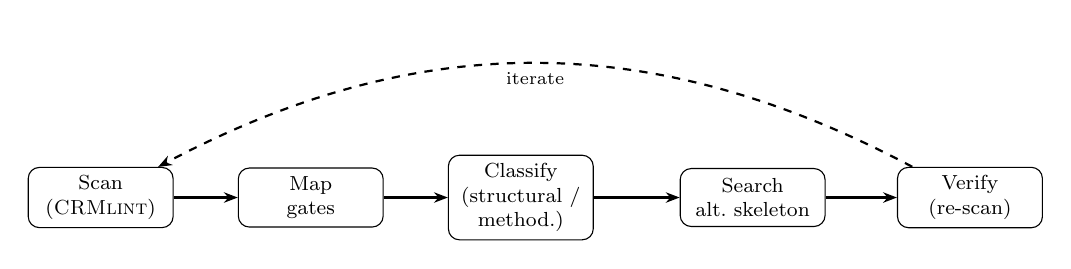
\begin{tikzpicture}[
    box/.style={draw, rounded corners, minimum width=2.0cm,
                minimum height=0.8cm, align=center, font=\footnotesize},
    arr/.style={-{Stealth[length=5pt]}, thick},
    >=Stealth,
    scale=0.92, transform shape
]
  \node[box] (scan) at (0,0) {Scan\\(\CRMlint)};
  \node[box] (map) at (2.9,0) {Map\\gates};
  \node[box] (classify) at (5.8,0) {Classify\\(structural /\\method.)};
  \node[box] (search) at (9.0,0) {Search\\alt.\ skeleton};
  \node[box] (verify) at (12.0,0) {Verify\\(re-scan)};

  \draw[arr] (scan) -- (map);
  \draw[arr] (map) -- (classify);
  \draw[arr] (classify) -- (search);
  \draw[arr] (search) -- (verify);
  \draw[arr, dashed] (verify) to[bend right=28] node[below,font=\scriptsize]
    {iterate} (scan);
\end{tikzpicture}
\caption{The scan-map-classify-search-verify loop.}
\label{fig:loop}
\end{figure}

In principle, the loop terminates: the CRM hierarchy is finite, so
the ceiling can only drop finitely many times.  In practice, we have
not executed this loop on any problem to completion.  The recipe is
a framework for thinking, not a demonstrated method.  Whether it
produces results that would not have been found by ordinary
mathematical intuition is an open question.


% ══════════════════════════════════════════════════════════════════════
%                           PART VIII
% ══════════════════════════════════════════════════════════════════════
\part{The Mathematics of the LTE}\label{part:math}

This part is expository.  We restate the main theorems of the LTE
in the form proved by Scholze, Commelin, and Massot, and annotate
each step with its CRM level.  Nothing here is new mathematics.
The proofs are theirs; the CRM labels are ours.  The labels may
be useful for readers approaching the LTE from the constructive
side, or for formalization teams deciding which components to
port to Lean~4.

\section{The main theorem and its reduction}\label{sec:main-thm}

The LTE establishes the following vanishing result, which
Scholze proposed as a challenge in December 2020.

\begin{theorem}[Clausen--Scholze {\cite{Scholze2020}}]\label{thm:lte-main}
Let $0 < p' < p \leq 1$ be real numbers, let $S$ be a profinite set,
and let $V$ be a $p$-Banach space.  Let $\mathcal{M}_{p'}(S)$ denote
the space of real $p'$-measures on~$S$.  Then
\[
  \mathrm{Ext}^i_{\mathrm{Cond}(\mathrm{Ab})}(\mathcal{M}_{p'}(S),\, V) = 0
  \qquad \text{for all } i \geq 1.
\]
\end{theorem}

The Ext-groups are computed in the abelian category of condensed
abelian groups.  The theorem says: from the perspective of homological
algebra in the condensed world, real-valued measures are
``projective-like'' --- they have no higher Ext against Banach targets.

\medskip
\noindent\textbf{CRM annotation.}
The \emph{statement} of Theorem~\ref{thm:lte-main} requires:
\begin{itemize}[nosep]
\item $p$-Banach space $V$: the norm $\|\cdot\|$ on $V$ satisfies
  $\|x + y\|^p \leq \|x\|^p + \|y\|^p$.  Defining
  this norm and its completeness is $\WLPO$.
\item The condensed abelian group $\mathcal{M}_{p'}(S)$:
  defined via a filtration $\mathcal{M}_{p'}(S)_{\leq c}$, each
  level a compact Hausdorff space.  The filtration cut-off is $\LPO$.
\item Profinite $S$: a cofiltered limit of finite sets.  All $\BISH$.
\end{itemize}

\noindent The \emph{proof} reduces Theorem~\ref{thm:lte-main} to a
chain of intermediate results, each of which we now state.

\section{The proof chain: six links}\label{sec:proof-chain}

The proof proceeds by six reductions, from the main theorem down to
the key technical result (Theorem~\ref{thm:94}).  We trace the full
chain and label each link with its CRM level.

\begin{center}
\small
\begin{tabular}{clll}
\toprule
\textbf{Link} & \textbf{Result} & \textbf{Mechanism} & \textbf{CRM} \\
\midrule
6 & Theorem~\ref{thm:lte-main} (main) &
  Long exact Ext sequence from Link~5 & $\BISH$ \\
5 & Ext-vanishing for $\mathcal{L}_{r'}(S)$ &
  $T^{-1}$-bijectivity via Link~4 & $\BISH$ \\
4 & Ext-vanishing for $\overline{\mathcal{L}}_{r'}(S)$ &
  Pro-isomorphism + derived limit via Link~3 & $\BISH$ \\
3 & Theorem~\ref{thm:94} (Ext-vanishing at finite level) &
  Double complex + spectral proposition & $\LPO$ \\
2 & Column exactness (Proposition~\ref{prop:col-exact}) &
  \v{C}ech nerve + normed snake lemma & $\LPO$ \\
1 & \v{C}ech exactness (Proposition~\ref{prop:cech-exact}) &
  Contracting homotopy + profinite limit & $\BISH$/$\WKL$ \\
\bottomrule
\end{tabular}
\end{center}

\subsection{Link 1: \v{C}ech nerve exactness ($\BISH$/$\WKL$)}

\begin{proposition}[\v{C}ech cover exactness {\cite{Commelin2022}}]
\label{prop:cech-exact}
Let $\pi: X \to B$ be a surjective morphism of profinite sets,
and let $S_\bullet \to S_{-1}$, $S_{-1} := B$, be its augmented
\v{C}ech nerve.  Let $V$ be a semi-normed group.  Then the complex
\[
  0 \longrightarrow \widehat{V}(S_{-1}) \longrightarrow
  \widehat{V}(S_0) \longrightarrow
  \widehat{V}(S_1) \longrightarrow \cdots
\]
is exact.  Moreover, for every $\varepsilon > 0$ and
$f \in \ker(\widehat{V}(S_m) \to \widehat{V}(S_{m+1}))$,
there exists $g \in \widehat{V}(S_{m-1})$ with $d(g) = f$
and $\|g\| \leq (1 + \varepsilon)\|f\|$.
\end{proposition}

\noindent\textbf{Proof sketch.}
For \emph{finite} $X$ and $B$, a section $\sigma: B \to X$ of $\pi$
induces maps $S_m \to S_{m+1}$ via
$(a_0, \ldots, a_m) \mapsto (\sigma(\pi(a_0)), a_0, \ldots, a_m)$.
These provide a contracting homotopy for the complex, and the homotopy
maps are norm-nonincreasing.  For general profinite sets, write
$X = \varprojlim_i X_i$ over its discrete (finite) quotients,
pass to finite quotients $X_i \to B_i$, apply the finite case, and
take the cofiltered limit.  Surjectivity of transition maps between
compact Hausdorff spaces is preserved under cofiltered limits
(by Tychonoff).

\medskip
\noindent\textbf{CRM annotation.}
The finite case is entirely $\BISH$: the section $\sigma$ exists
because $\pi$ is surjective between finite sets, and the contracting
homotopy is an explicit combinatorial construction.  The passage to
profinite limits uses Tychonoff's theorem for compact Hausdorff spaces
(surjections of compact spaces remain surjective under cofiltered
limits).  In CRM terms, Tychonoff for Hausdorff spaces is $\WKL$
(equivalent to weak K\"onig's lemma: an infinite finitely-branching
tree has an infinite path).  The norm estimates ($\|g\| \leq
(1+\varepsilon)\|f\|$) do not introduce additional logical cost.

\subsection{Link 2: Column exactness via normed snake lemma ($\LPO$)}

The double complex construction requires that each column is
``weakly bounded exact.''  This is established by combining
\v{C}ech exactness (Link~1) with the normed $T^{-1}$-action.

\begin{definition}[Weak bounded exactness {\cite{Commelin2022}}]
\label{def:weak-exact}
A system of complexes $C_\bullet^\bullet$ is
\emph{weakly $\leq k$-exact in degrees $\leq m$ for $c \geq c_0$
with bound~$K$} if for all $c \geq c_0$, all $x \in C_{kc}^i$ with
$i \leq m$, and any $\varepsilon > 0$, there exists $y \in C_c^{i-1}$
with
\[
  \|x_{|c} - dy\| \leq K\|dx\| + \varepsilon.
\]
\end{definition}

\begin{proposition}[Column exactness {\cite{Commelin2022}}]
\label{prop:col-exact}
Let $k > 1$, $c_0 > 0$ with $(k-1)c_0/N \geq d$ (the splittability
error).  Let $m$ be any natural number, and put
\[
  K = (m+2) + \frac{r+1}{r(1-r)}(m+2)^2.
\]
Then the $i$-th column in the double complex is $(k^2, K)$-weakly
bounded exact in degrees $\leq m$ for $c \geq c_0'$.
\end{proposition}

\noindent\textbf{Proof sketch.}
The key input is the ``normed dual snake lemma''
(Proposition~\ref{prop:snake} below): given two admissible systems of
complexes $M_\bullet^\bullet$ and ${M'}_\bullet^\bullet$ with a map
$f: M \to M'$, if both $M$ and $M'$ are weakly bounded exact, then
the kernel complex inherits weak bounded exactness (with controlled
loss in the constants).  The column is built from the Čech nerve of
the summation map $M^N_{c/N} \to M_c$, and the $T^{-1}$-action
introduces the norm scaling.

\medskip
\noindent\textbf{CRM annotation.}
The splittability lemma ($N$-splittability of $\mathrm{Hom}(\Lambda,
\overline{\mathcal{L}}_{r'}(S))$) is $\BISH$: it decomposes elements
of a polyhedral lattice module into $N$ pieces of roughly $1/N$-th
the norm.  The column exactness proof combines this with the $\LPO$
content of the filtration cut-offs $M_{\leq c}$.  The constant~$K$
depends on $m$ and $r$ (not on the profinite set $S$ or the normed
module $V$), so the ``universal'' part of the proof is $\BISH$ and
the $\LPO$ enters only at the interface where elements are tested
against filtration levels.

\subsection{Link 3: The key technical result ($\LPO$)}

\begin{theorem}[Theorem 9.4 {\cite{Scholze2019, Commelin2022}}]
\label{thm:94}
Let $\mathrm{BD} = (n, f, h)$ be a Breen--Deligne package, and let
$\kappa = (\kappa_0, \kappa_1, \ldots)$ be a sequence of constants
in $\R_{\geq 0}$ that is $\mathrm{BD}$-suitable.  Fix radii
$1 > r' > r > 0$.  For any $m$ there exist $k$ and $c_0$ such that
for all profinite sets $S$ and all $r$-normed
$\Z[T^{\pm 1}]$-modules~$V$, the system of complexes
\[
  C^{\mathrm{BD}}_\kappa(\overline{\mathcal{L}}_{r'}(S))^\bullet_c
  \colon \;
  \widehat{V}(\overline{\mathcal{L}}_{r'}(S)_{\leq c})^{T^{-1}}
  \longrightarrow
  \widehat{V}(\overline{\mathcal{L}}_{r'}(S)_{\leq \kappa_1 c}^2)^{T^{-1}}
  \longrightarrow \cdots
\]
is $\leq k$-exact in degrees $\leq m$ for $c \geq c_0$.
\end{theorem}

\noindent\textbf{Proof structure.}
The proof is by induction on $m$.  The inductive step requires a
\emph{stronger} statement (Theorem~9.5$'$ in the blueprint), which
introduces a polyhedral lattice $\Lambda$ and replaces
$\overline{\mathcal{L}}_{r'}(S)$ by
$\mathrm{Hom}(\Lambda, \overline{\mathcal{L}}_{r'}(S))$.
Theorem~\ref{thm:94} is recovered by setting $\Lambda = \Z$.

The inductive step constructs a \emph{system of double complexes}:
\begin{enumerate}[nosep]
\item \textbf{Rows:} Apply the Breen--Deligne system functor to
  $\mathrm{Hom}(\Lambda^{(\bullet)}, M)$, where $\Lambda^{(\bullet)}$
  is the cosimplicial polyhedral lattice and $M$ abbreviates
  $\overline{\mathcal{L}}_{r'}(S)$.  Take the alternating face map
  complex.  Rescale norms by $m!$ for admissibility.
\item \textbf{Columns:} The column at index~$i$ is the Čech nerve
  construction of Link~2, applied with the $i$-th Breen--Deligne data.
\item \textbf{Homotopy:} The Breen--Deligne homotopy $h^N$ (the
  $N$-fold composition of the package's built-in homotopy) provides
  maps $M^{0,q+1}_{k'c} \to M^{1,q}_c$ bounded by some constant~$H$.
  The ``homotopic map'' $\delta^{0,q}_c$ factors through a deep
  restriction and has norm $\leq \varepsilon$.
\end{enumerate}

\noindent The three ingredients (row exactness by induction, column
exactness from Link~2, homotopy condition) are fed into the
\emph{spectral proposition} (Proposition~\ref{prop:spectral} below),
which yields weak bounded exactness of the first row---completing
the induction.

\medskip
\noindent\textbf{CRM annotation.}
The double complex construction (cosimplicial lattice, alternating
face map, norm rescaling) is $\BISH$: it is combinatorial algebra
over $\Z$.  The Breen--Deligne resolution itself is $\BISH$: it is a
functorial resolution of abelian groups by free modules, specified by
integer matrices.  The homotopy bound~$H$ is computed from the
Breen--Deligne data and $r, r'$---a finite computation over $\Q$,
hence $\BISH$.

The $\LPO$ enters at two points: (i) the filtration cut-offs
$\overline{\mathcal{L}}_{r'}(S)_{\leq c}$ in the system of complexes,
and (ii) the norm estimate $r^b N \leq \varepsilon$ (choosing $b$
so that $2k'(r/r')^b \leq \varepsilon$), which requires comparing
real numbers.  The choice of $N$ as a power of~2 satisfying
$k'/N \leq (r')^b$ is a single $\LPO$ decision on the ordered
reals.

\subsection{Links 4--6: Algebraic reductions ($\BISH$)}

\noindent\textbf{Link 4: From finite level to $\overline{\mathcal{L}}_{r'}(S)$.}
Write $Q'(\overline{\mathcal{M}}_{r'}(S)) = \varinjlim_c
Q'(\overline{\mathcal{M}}_{r'}(S))_{\leq c}$ and reduce to a
pro-isomorphism statement at each finite level.  The passage to the
derived limit uses a resolution
$0 \to \bigoplus_n Q'_{\leq n} \to \bigoplus_n Q'_{\leq n} \to
Q' \to 0$
and checks that the relevant squares are bicartesian (vertical kernels
and cokernels form pro-zero systems).  This is diagram chasing in
$\mathrm{Cond}(\mathrm{Ab})$, entirely $\BISH$.

\medskip
\noindent\textbf{Link 5: From $\overline{\mathcal{L}}_{r'}(S)$
to $\mathcal{L}_{r'}(S)$.}
The short exact sequence
\[
  0 \longrightarrow \Z[T^{-1}][S] \longrightarrow
  \mathcal{L}_{r'}(S) \longrightarrow
  \overline{\mathcal{L}}_{r'}(S) \longrightarrow 0
\]
decomposes Laurent measures into negative and positive parts.
Apply $\mathrm{Ext}^*(\_, V)$: the $\Z[T^{-1}][S]$-term has
vanishing higher Ext (because $\Z[S]$ is free), and the
$\overline{\mathcal{L}}_{r'}(S)$-term vanishes by Link~4.
The five lemma gives vanishing for $\mathcal{L}_{r'}(S)$.
This is abstract homological algebra, all $\BISH$.

\medskip
\noindent\textbf{Link 6: Main theorem.}
The short exact sequence
\[
  0 \longrightarrow \mathcal{L}_{r'}(S) \xrightarrow{2T-1}
  \mathcal{L}_{r'}(S) \longrightarrow
  \mathcal{M}_{p'}(S) \longrightarrow 0
\]
(evaluation at $T = 1/2$) reduces the main theorem to the Ext-vanishing
of $\mathcal{L}_{r'}(S)$ from Link~5 via the long exact sequence.
The surjectivity of evaluation at $T = 1/2$ on pseudo-normed groups
is a norm estimate (strong exactness), which uses
Tychonoff ($\WKL$) for passage to profinite limits.  But the
long-exact-sequence argument itself is $\BISH$.


\section{The normed homological algebra toolkit}\label{sec:toolkit}

The LTE's main technical innovation is not the theorem statement
but the \emph{toolkit}: a library of normed homological algebra
results with explicit quantitative control.  These results are
general-purpose and transfer directly to other formalization targets.

\subsection{Controlled surjectivity}

\begin{lemma}[Closure surjectivity {\cite{Commelin2022}}]
\label{lem:closure-surj}
Let $G$ and $H$ be normed groups, $K \leq H$ a subgroup, and
$f: G \to H$ a $C$-surjective morphism onto $K$ (i.e., for all
$x \in K$ there exists $g$ with $f(g) = x$ and
$\|g\| \leq C\|x\|$).  If $G$ is complete, then $f$ is
$(C+\varepsilon)$-surjective onto $\overline{K}$ for every
$\varepsilon > 0$.
\end{lemma}

\noindent\textbf{Proof idea.}
Write $x \in \overline{K}$ as $x = \sum_{i \geq 0} x_i$ with
$x_i \in K$ and $\|x_i\| \leq \varepsilon_i$ for a rapidly
decreasing sequence.  Lift each $x_i$ to $g_i$ with
$\|g_i\| \leq C\|x_i\|$, and set $g = \sum g_i$.  Completeness
of $G$ guarantees convergence.  The norm estimate
$\|g\| \leq (C+\varepsilon)\|x\|$ follows from the geometric
series bound on the $\varepsilon_i$.

\medskip
\noindent\textbf{CRM annotation.}
The proof uses completeness of $G$ (to sum the Cauchy series
$\sum g_i$), which is $\WLPO$ (Cauchy convergence test).  The
lifting $x_i \mapsto g_i$ uses the $C$-surjectivity hypothesis,
which is $\BISH$ (explicit choice of lifts).  The norm comparison
$\|g_i\| \leq C\|x_i\|$ is an inequality between real numbers
($\LPO$).

\subsection{Controlled exactness}

\begin{lemma}[Controlled exactness {\cite{Commelin2022}}]
\label{lem:controlled-exact}
Let $f: M_0 \to M_1$ and $g: M_1 \to M_2$ be bounded maps between
normed groups.  Suppose $f$ is $C$-surjective onto $\ker g$, and
$g$ is $D$-surjective onto its image.  Then for every
$\varepsilon > 0$, the completion $\widehat{f}$ is
$(C+\varepsilon)$-surjective onto $\ker \widehat{g}$.
\end{lemma}

\noindent This is the mechanism by which the LTE passes from
``incomplete'' exactness (at the pre-completion level, $\BISH$) to
``completed'' exactness (at the normed-completion level, $\WLPO$).
The upgrade is Lemma~\ref{lem:closure-surj} applied to $K = \ker g$
inside $\widehat{M_1}$.

\subsection{The normed snake lemma}

\begin{proposition}[Weak normed snake lemma {\cite{Commelin2022}}]
\label{prop:snake}
Let $M_\bullet^\bullet$ and ${M'}_\bullet^\bullet$ be two admissible
systems of complexes of complete normed abelian groups, with a
norm-nonincreasing map $f: M \to M'$ satisfying
$\|x_{|c}\| \leq K'' \|f(x)\|$ for all $x \in M^i_{k''c}$,
$i \leq m+1$.  If $M$ is weakly $\leq k$-exact with bound~$K$
and $M'$ is weakly $\leq k'$-exact with bound~$K'$, then the
quotient $N = M'/M$ is weakly $\leq kk'k''$-exact in degrees
$\leq m-1$ with bound $K'(KK''+1)$.
\end{proposition}

\noindent\textbf{CRM annotation.}
The proof is a quantitative diagram chase: lift $n \in N^i$ to
$m' \in M'^i$, decompose $dm'$ using the quotient norm, apply
weak exactness of $M$ and $M'$, and track constants through.
The diagram chase is $\BISH$; the norm estimates are $\LPO$.
The bound $K'(KK''+1)$ is explicit and computable.

The \emph{dual} snake lemma (for kernels instead of cokernels)
is proved analogously, with bound $K + r_1 r_2 K K'$.
Both versions are used in the inductive step of Theorem~\ref{thm:94}:
the snake lemma produces column exactness,
and the dual snake lemma produces the kernel
complex for the $T^{-1}$-action.

\subsection{The spectral proposition}

\begin{proposition}[Spectral proposition {\cite{Commelin2022}}]
\label{prop:spectral}
Fix $m \geq 0$ and constants $k, K$.  There exist $\varepsilon > 0$
and $k_0, K_0$ (depending only on $k, K, m$) such that: if
a system of double complexes $M^{p,q}_c$ is admissible and satisfies
\begin{enumerate}[nosep,label=(\roman*)]
\item rows are weakly $\leq k$-exact in degrees $\leq m-1$ with
  bound~$K$ (for $i = 0, \ldots, m+1$),
\item columns are weakly $\leq k$-exact in degrees $\leq m$ with
  bound~$K$,
\item the normed spectral homotopy condition for $m$, some $H > 0$,
  $c_0$, and~$\varepsilon$,
\end{enumerate}
then the first row is weakly $\leq k'^2$-exact in degrees $\leq m$
with bound $2K_0 H$.
\end{proposition}

\noindent This is the engine of the induction.  The base case ($m=0$)
uses $\varepsilon = 1/(2k)$ and the homotopy condition to absorb the
$\varepsilon$-term.  The inductive step passes to the quotient complex
$N^{p,0} = M^{p,1}/\overline{M^{p,0}}$ and applies the snake lemma
(Proposition~\ref{prop:snake}) to verify the hypotheses for $m-1$.

\medskip
\noindent\textbf{CRM annotation.}
The spectral proposition is $\BISH$ in its logical content: it is a
statement about constants and admissibility conditions.  The $\LPO$
enters only when the proposition is \emph{applied} to a specific
system of double complexes built from normed groups.  This separation
is a paradigm case of the concentration thesis: the abstract machinery
is logically free, and the analytic cost is paid only at the
point of application.


\section{The Breen--Deligne resolution: pure algebra}\label{sec:BD}

The deepest algebraic ingredient in the LTE is the Breen--Deligne
resolution, which provides a functorial free resolution of any
abelian group~$A$.

\begin{theorem}[Breen--Deligne {\cite{BreenDeligne}}]
For any abelian group $A$, there is a resolution, functorial in~$A$:
\[
  \cdots \longrightarrow \bigoplus_{i} \Z[A^{r_{ij}}]
  \longrightarrow \cdots
  \longrightarrow \Z[A^3] \oplus \Z[A^2]
  \longrightarrow \Z[A^2]
  \longrightarrow \Z[A]
  \longrightarrow A \longrightarrow 0.
\]
The functorial maps $\Z[A^m] \to \Z[A^n]$ are specified by
integer matrices (``basic universal maps'': $n \times m$ matrices
over $\Z$), composed via matrix multiplication.
\end{theorem}

\noindent\textbf{CRM annotation.}
The entire Breen--Deligne resolution---its existence, functoriality,
and the universal maps---is $\BISH$.  The universal maps are
$\Z$-linear combinations of basic universal maps specified by
integer matrices; their composition is matrix multiplication; the
homotopy $h$ packaged with the resolution is a universal map bounded
by an integer~$N$.  No real analysis, no completeness, no decidability
of real arithmetic appears anywhere.

This is the algebraic skeleton of the LTE in its purest form.
The LTE formalizes it in Lean~3 as
\texttt{breen\_deligne.basic\_universal\_map} (integer matrices),
\texttt{breen\_deligne.universal\_map} (formal $\Z$-linear
combinations), and \texttt{breen\_deligne.package} (the triple
$(n, f, h)$).

\section{What transfers: reusable components}\label{sec:reusable}

The LTE's mathematical infrastructure divides into three categories
by reusability.

\subsection{Category A: Directly reusable ($\BISH$)}

These components depend on no analytic input and can be ported to
Lean~4 as standalone libraries.

\begin{enumerate}[nosep]
\item \textbf{Breen--Deligne package.}  Integer matrices, universal
  maps, the package triple $(n, f, h)$, homotopy composition
  $h^N$, suitability conditions on $\kappa$.  All finitary
  algebra over $\Z$.

\item \textbf{Polyhedral lattices.}  Finite free abelian groups with
  generating norms.  The key combinatorial lemma:
  $N$-splittability of $\mathrm{Hom}(\Lambda,
  \overline{\mathcal{L}}_{r'}(S))$ with explicit error term~$d$.

\item \textbf{Cosimplicial polyhedral lattices.}
  $\Lambda' = \Lambda^N$ with the $\ell^1$-norm; the cosimplicial
  object $\Lambda^{(\bullet)}$; the Čech nerve isomorphisms
  $\mathrm{Hom}(\Lambda'^{(m)}, M)_{\leq c} \cong
  \mathrm{Hom}(\Lambda', M)_{\leq c}^{m /
  \mathrm{Hom}(\Lambda, M)_{\leq c}}$.

\item \textbf{Abstract diagram chasing.}  The pro-isomorphism
  argument (Link~4), the five-lemma reduction (Link~5), the
  short-exact-sequence reduction (Link~6).
\end{enumerate}

\subsection{Category B: Reusable with $\LPO$ interface ($\LPO$)}

These components are algebraic in structure but require norm
comparisons at the interface.

\begin{enumerate}[nosep]
\item \textbf{Systems of complexes.}  Functors
  $(\R_{\geq 0})^{\mathrm{op}} \to \mathrm{Ch}(\mathrm{SemiNormGrp})$.
  The restriction maps $\mathrm{res}_{c',c}$ require
  $c' \geq c$ ($\LPO$).  The definitions of $\leq k$-exactness,
  weak $\leq k$-exactness, and admissibility are $\BISH$
  conditions on the norms.

\item \textbf{The spectral proposition.}
  The statement and proof of Proposition~\ref{prop:spectral}
  are $\BISH$ as abstract algebra.  The $\LPO$ enters only at
  instantiation.

\item \textbf{The normed snake lemma (both versions).}
  The diagram chase is $\BISH$; the norm bounds use
  $\LPO$.
\end{enumerate}

\subsection{Category C: Analytic core ($\WLPO$/$\LPO$)}

These components are irreducibly analytic.

\begin{enumerate}[nosep]
\item \textbf{Normed completions $\widehat{V}(\cdot)$.}
  The completion functor on semi-normed groups.  Cauchy
  convergence is $\WLPO$; the norm on the completion is $\LPO$.

\item \textbf{The $T^{-1}$-action on $\overline{\mathcal{L}}_{r'}(S)$.}
  The shift $T^{-1} \cdot (\sum a_n T^n) = (\sum a_{n+1} T^n)$
  scales the norm by $r'$: the filtration level changes from
  $\leq c$ to $\leq c/r'$.  This scaling requires norm
  comparison ($\LPO$).

\item \textbf{The homotopy norm estimate.}
  The key bound $r^b N \leq \varepsilon$ (choosing $b$ so that
  $2k'(r/r')^b \leq \varepsilon$) requires decidable ordering
  on $\R$ ($\LPO$).  This is the deepest analytic content in
  the entire proof: a single real-number comparison that
  controls the convergence of the induction.
\end{enumerate}

\section{Lean~4 formalization targets}\label{sec:lean4}

The LTE was formalized in Lean~3 (community \texttt{mathlib} fork).
A Lean~4 port faces the standard Lean~3 $\to$ Lean~4 translation
burden, but the \emph{mathematical} targets are well-defined.
We identify the most valuable targets from the CRM perspective:
components where the $\BISH$/$\LPO$ separation is sharpest and
the reuse potential is highest.

\subsection{Target 1: Breen--Deligne package (pure $\BISH$)}

\begin{verbatim}
-- Basic universal maps: integer matrices
structure BasicUniversalMap (m n : Nat) where
  matrix : Matrix (Fin n) (Fin m) Int

-- Universal maps: formal Z-linear combinations
structure UniversalMap (m n : Nat) where
  terms : List (Int x BasicUniversalMap m n)

-- Composition via matrix multiplication
def UniversalMap.comp (f : UniversalMap m n)
    (g : UniversalMap l m) : UniversalMap l n := ...

-- BD package: exponents, differentials, homotopy
structure BDPackage where
  n : Nat -> Nat                  -- exponents
  f : (i : Nat) -> UniversalMap (n (i+1)) (n i)
  h : (i : Nat) -> UniversalMap (n (i+1)) (n i)
  chain_complex : forall i, (f i).comp (f (i+1)) = 0
  homotopy_rel : forall i, ...   -- h witnesses null-homotopy
\end{verbatim}

This is finite combinatorics over $\Z$.  No axioms beyond
\texttt{propext} and \texttt{Quot.sound}.  The key theorem to
formalize: given a BD package and a suitable sequence $\kappa$,
the $N$-fold homotopy $h^N$ exists and is bounded by an explicit
integer.

\subsection{Target 2: Systems of complexes ($\BISH$ definitions, $\LPO$ at interface)}

\begin{verbatim}
-- System of complexes: parametrized by NNReal
structure SystemOfComplexes where
  C : NNReal -> ChainComplex SemiNormedGroup
  res : forall c' c, c' >= c -> C c' --> C c
  res_comp : forall c'' c' c (h1 : c'' >= c')
    (h2 : c' >= c), res c'' c (le_trans h2 h1) =
    (res c' c h2).comp (res c'' c' h1)

-- Weak bounded exactness
def SystemOfComplexes.IsWeakBoundedExact
    (S : SystemOfComplexes) (k K : Real) (m : Nat)
    (c0 : NNReal) : Prop :=
  forall c >= c0, forall i <= m,
    forall x in (S.C (k * c)).obj i,
    forall eps > 0, exists y in (S.C c).obj (i-1),
      norm (res x - d y) <= K * norm (d x) + eps
\end{verbatim}

The definition is $\BISH$.  The $\LPO$ enters at the inequality
$c' \geq c$ (comparison of real numbers) and the norm estimate.

\subsection{Target 3: Controlled surjectivity lemma ($\WLPO$)}

\begin{verbatim}
-- Key lemma: C-surjectivity extends to closures
theorem controlled_closure_of_complete
    {G H : NormedAddCommGroup} [CompleteSpace G]
    {K : AddSubgroup H} {f : G ->+ H} {C : Real}
    (hf : forall x in K,
      exists g, f g = x && norm g <= C * norm x)
    (eps : Real) (heps : 0 < eps) :
    forall x in K.topologicalClosure,
      exists g, f g = x
        && norm g <= (C + eps) * norm x := by
  -- Proof: geometric series in complete G
  ...
\end{verbatim}

This requires \texttt{CompleteSpace G} ($\WLPO$: Cauchy sequences
converge) and the norm bound ($\LPO$: $\|g\| \leq C\|x\|$).
The Lean~4 proof would use \texttt{Metric.cauchySeq\_of\_le\_geometric}
from Mathlib.

\subsection{Target 4: Normed snake lemma ($\BISH$ chase, $\LPO$ bounds)}

The most technically demanding target.  The Lean~3 proof
(\texttt{weak\_normed\_snake} and \texttt{weak\_normed\_snake\_dual})
runs approximately 200 lines.  A Lean~4 port would:
\begin{itemize}[nosep]
\item Define admissible systems of complexes over Mathlib's
  \texttt{SemiNormedGroup}.
\item Implement the quantitative diagram chase with explicit
  $\varepsilon$-management.
\item Prove the bound $K'(KK''+1)$ for quotients and
  $K + r_1 r_2 K K'$ for kernels.
\end{itemize}

The entire chase is $\BISH$ (diagram manipulation in an abelian
category with explicit lifts).  The $\LPO$ enters only at the
final norm inequality.

\subsection{CRM summary of formalization targets}

\begin{center}
\begin{tabular}{llcl}
\toprule
\textbf{Target} & \textbf{Component} & \textbf{CRM} & \textbf{Lean~4 difficulty} \\
\midrule
1 & Breen--Deligne package  & $\BISH$ & Low (finite algebra over $\Z$) \\
2 & Systems of complexes    & $\BISH$/$\LPO$ & Medium (parametrized complexes) \\
3 & Controlled surjectivity & $\WLPO$ & Low (standard Cauchy argument) \\
4 & Normed snake lemma      & $\BISH$/$\LPO$ & High (200-line diagram chase) \\
\bottomrule
\end{tabular}
\end{center}

Targets~1 and~3 are low-hanging fruit: they are self-contained,
well-typed, and already have Lean~3 implementations to translate.
Target~2 requires design decisions about how to interface
with Mathlib's \texttt{CategoryTheory.ChainComplex}.
Target~4 is the highest-value formalization: the normed snake
lemma is the engine of the induction, and a clean Lean~4
version would serve as infrastructure for any future normed
homological algebra project.


% ══════════════════════════════════════════════════════════════════════
%                       ACKNOWLEDGMENTS
% ══════════════════════════════════════════════════════════════════════

\section*{Acknowledgments}

The LTE blueprint \texttt{.tex} files used in Parts~IV and~VIII were
authored by Johan Commelin and Patrick Massot as part of the Liquid
Tensor Experiment, available at
\url{https://github.com/leanprover-community/liquid}.
The mathematical content of Part~VIII follows the proofs in
\cite{Scholze2019} as formalized in \cite{Commelin2022}.
The CRM programme (Papers 1--98) is the author's independent work;
\CRMlint\ was developed with AI assistance (Claude, Anthropic).
No funding was received for this work.


% ══════════════════════════════════════════════════════════════════════
%                         REFERENCES
% ══════════════════════════════════════════════════════════════════════
\begin{thebibliography}{99}

\bibitem{Bishop1967}
E.~Bishop,
\emph{Foundations of Constructive Analysis},
McGraw-Hill, 1967.

\bibitem{BridgesRichman1987}
D.~Bridges and F.~Richman,
\emph{Varieties of Constructive Mathematics},
London Mathematical Society Lecture Note Series~97,
Cambridge University Press, 1987.

\bibitem{Scholze2019}
P.~Scholze,
\emph{Lectures on Analytic Geometry},
Bonn lecture notes, 2019.
Available at \url{https://www.math.uni-bonn.de/people/scholze/Analytic.pdf}.

\bibitem{Scholze2020}
P.~Scholze,
Liquid tensor experiment,
\emph{Experimental Mathematics} (challenge post), December 2020.

\bibitem{Commelin2022}
J.~Commelin and P.~Massot,
Liquid Tensor Experiment: formal verification in Lean~3,
2022.
Repository: \url{https://github.com/leanprover-community/liquid}.

\bibitem{ClausenScholze2022}
D.~Clausen and P.~Scholze,
\emph{Condensed Mathematics and Complex Geometry},
2022.

\bibitem{Lee_P5}
P.~C.-K.~Lee,
General relativity is $\BISH + \LPO$: the logical cost of the
equivalence principle,
Paper~5, CRM Series, 2024.
DOI: \texttt{10.5281/zenodo.18765700}.

\bibitem{Lee_P72}
P.~C.-K.~Lee,
The DPT Characterisation Theorem,
Paper~72, CRM Series, 2025.

\bibitem{Lee_P73}
P.~C.-K.~Lee,
Axiom~1 is irreversible,
Paper~73, CRM Series, 2025.

\bibitem{Lee_P74}
P.~C.-K.~Lee,
Axiom~2 is irreversible,
Paper~74, CRM Series, 2025.

\bibitem{Lee_P76}
P.~C.-K.~Lee,
CRMLint: Automated CRM logical cost analyzer,
Paper~76, CRM Series, 2026.
DOI: \texttt{10.5281/zenodo.18779362}.

\bibitem{Lee_P77}
P.~C.-K.~Lee,
Explicit Hodge decompositions for $E^4$,
Paper~77, CRM Series, 2026.
DOI: \texttt{10.5281/zenodo.18777596}.

\bibitem{Lee_P78}
P.~C.-K.~Lee,
The Local Langlands Correspondence for $\mathrm{GL}_2(\Q_2)$
is constructively decidable,
Paper~78, CRM Series, 2026.
DOI: \texttt{10.5281/zenodo.18789008}.

\bibitem{Lee_P90}
P.~C.-K.~Lee,
The Squeeze is a Microscope: Automated Constructivization from
CRMLint to the Hodge Horizon,
Paper~90, CRM Series, 2026.
DOI: \texttt{10.5281/zenodo.18809911}.

\bibitem{Lee_P95}
P.~C.-K.~Lee,
The BSD Squeeze: CRMLint Decomposition of the Gross--Zagier--Kolyvagin
Proof,
Paper~95, CRM Series, 2026.
DOI: \texttt{10.5281/zenodo.18821019}.

\bibitem{Lee_P96}
P.~C.-K.~Lee,
The Root Number Bifurcation: CRM Cost of BSD Detection Controlled
by the Functional Equation,
Paper~96, CRM Series, 2026.
DOI: \texttt{10.5281/zenodo.18869924}.

\bibitem{Lee_P98}
P.~C.-K.~Lee,
The Motivic CRM Architecture,
Paper~98, CRM Series, 2026.

\bibitem{Mathlib}
The Mathlib Community,
\emph{Mathlib4: Mathematics in Lean~4},
\url{https://github.com/leanprover-community/mathlib4}, 2024--2026.

\bibitem{Simpson2009}
S.~G.~Simpson,
\emph{Subsystems of Second Order Arithmetic},
2nd ed., Cambridge University Press, 2009.

\bibitem{BreenDeligne}
L.~Breen,
Extensions du groupe additif,
\emph{Inst.\ Hautes \'Etudes Sci.\ Publ.\ Math.}~48 (1978), 39--125.

\bibitem{Tychonoff1930}
A.~N.~Tychonoff,
\"Uber die topologische Erweiterung von R\"aumen,
\emph{Math.\ Ann.}~102 (1930), 544--561.

\end{thebibliography}

\end{document}
